\ifx\allfiles\undefined
\documentclass{beamer}
\usepackage{xeCJK}
\setmonofont[Mapping={}]{JetBrains Mono}
\setmainfont{JetBrains Mono}
\setsansfont{JetBrains Mono}
\setCJKmainfont{微軟正黑體}
\setCJKsansfont{微軟正黑體}
\usetheme[secheader]{Boadilla}
%\usepackage{ctable} % 表格
\usepackage{color} % 字體顏色
\usepackage{hyperref}
\usepackage{listings} % 程式碼區塊用
\lstset{
	language=Java,
	showtabs=false,
	showstringspaces=false
}
\begin{document}
\input{setting/command}
\fi
%----------------------------
%----------------------------
\section{專案結構}
\subsection{Test Explorer 概覽}
\begin{frame}
    \frametitle{專案結構}
    \begin{columns}
        \column{.5\textwidth}
        以下{\color{red}紅色}為付費升級版功能
        \begin{itemize}
            \item \hyperlink{profiles}{Profiles}
            \item Test Cases
            \item \hyperlink{objectRepository}{Object Repository}
            \item \hyperlink{dataFile}{Data Files}
            \item { \color{red} 
                Checkpoints
            }
            \item  \hyperlink{keywords}{Keywords}
            \item Test Listener
            \item { \color{red} 
                \hyperlink{reports}{Reports}
            }
            \item TestOps
            \item Include
            \item Plugins
        \end{itemize}
        \column{.5\textwidth}
        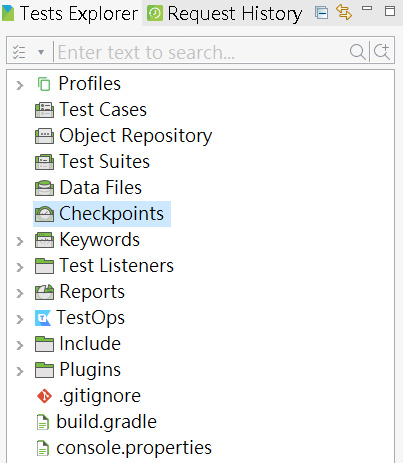
\includegraphics[height=0.75\textheight]{picture/專案結構.jpg}
    \end{columns}
\end{frame}	
%----------------------------
\label{profiles}
\subsection{Profiles}
\begin{frame}[fragile]
    \frametitle{Profiles}
    % -- Code block--
    \begin{block}{Profiles設定值引用}
\begin{lstlisting}
import internal.GlobalVariable
GlobalVariable.varibleName
\end{lstlisting}
    \end{block}
    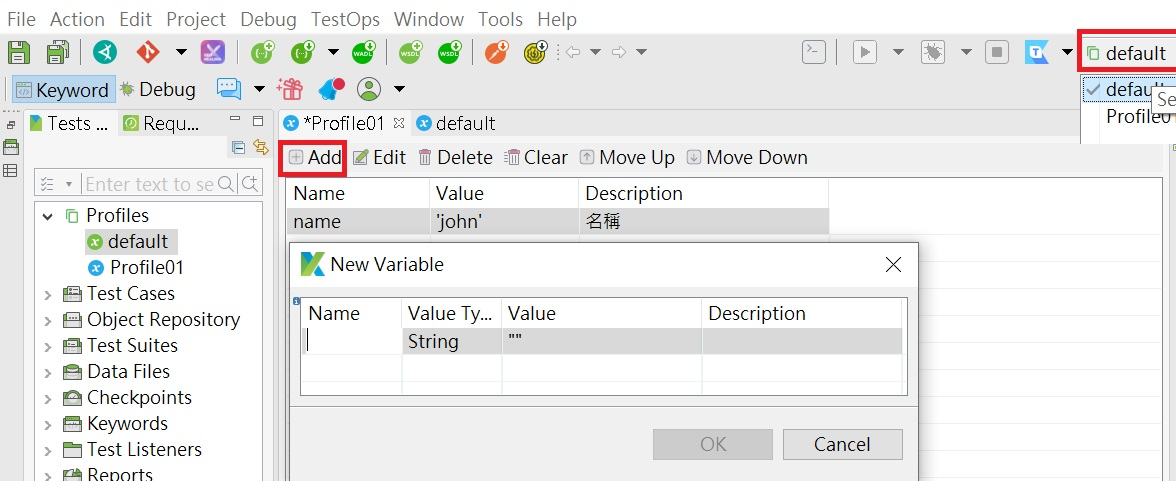
\includegraphics[width=1\textwidth]{picture/Profile新增數值.jpg}
\end{frame}
%----------------------------
\label{objectRepository}
\subsection{Object Repository}
\begin{frame}
    \frametitle{Object Repository}
    Request 物件可以使用變數替代字串方便切環境,寫法為\$\{varibleName\},
    記得切 tab 前要儲存不然已經寫上去的內容會立刻消失。
    %\hyperlink{gstring}{\beamerbutton{gstring}} 
    ~\\
    可以搭配 Profile 中設定的變數做環境設定值切換。
    ~\\~\\
    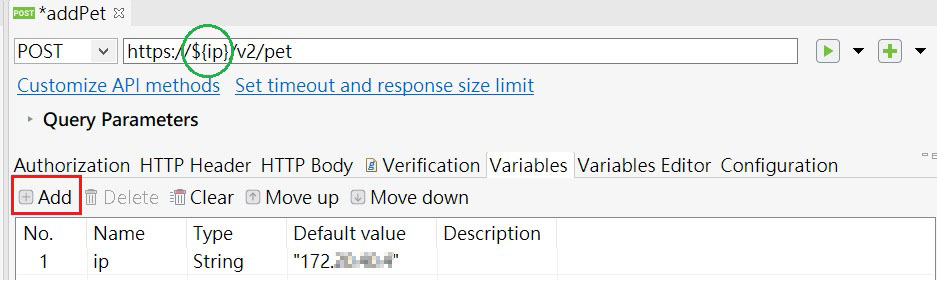
\includegraphics[width=1\textwidth]{picture/addVarible.jpg}
\end{frame}
%----------------------------
\begin{frame}
    \frametitle{Object Repository}
    如果已經有使用 Postman 或者 SoapUI 建立過 Request 也可以直接匯入。
    \begin{center}
        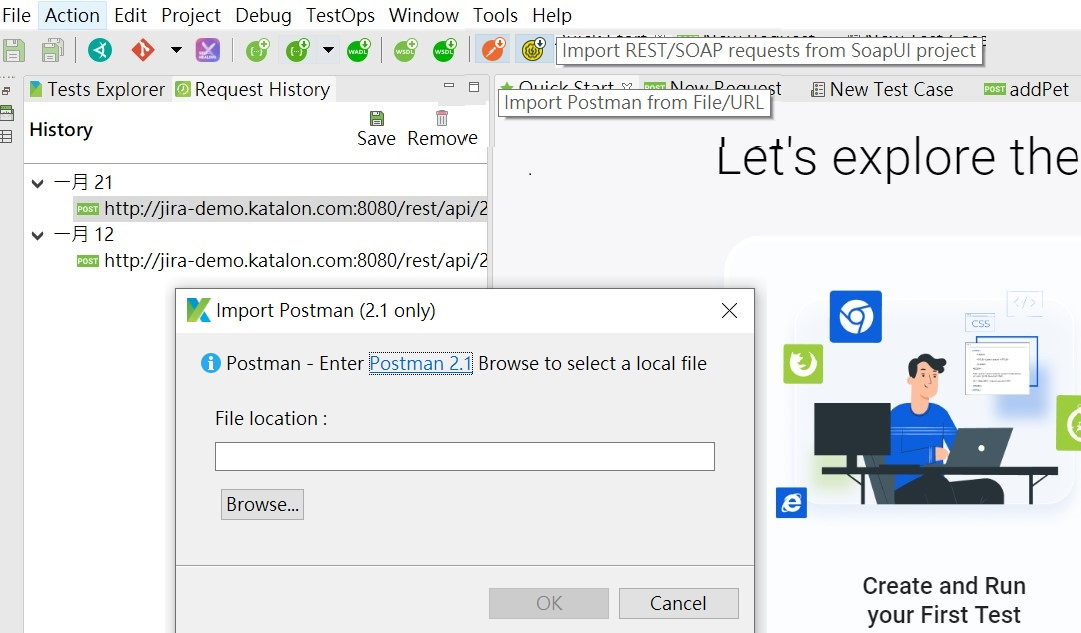
\includegraphics[width=0.9\textwidth]{picture/importRequest.jpg}
    \end{center}
\end{frame}
%----------------------------
\label{dataFile}
\subsection{Data File}
\begin{frame}
	\frametitle{Data Files}
	\begin{block}{測試資料產生的放置位置}
		專案目錄/Data Files/
	\end{block}
	自訂的測試資料檔案(csv/excel)可以不用放這裡,可以設定相對路徑讀取
    \begin{center}
        \includegraphics[width=0.57\textwidth]{picture/example/Data.jpg}
    \end{center}
\end{frame}
%----------------------------
\label{keywords}
\subsection{Keywords}
\begin{frame}
    \frametitle{Keywords}
    所有的自訂 Groovy 類別可以寫在這裡,
    可以直接由 Test Case Script 中直接import使用。
    ~\\~\\
    這裡僅有 Groovy 檔案會顯示出來,
    例如 privateKey.pem 這種檔案就不會顯示,
    但還是可以直接進專案目錄放置該檔案並於Script中讀取。\\
    有讀取 classpath 中檔案需求可以留意。
    ~\\~\\
    如果不是要自訂groovy 類別而是用第三方 library,
    例如:Gson、HikariCP、Jedis ,
    可以將該Jar檔案放到下列目錄裡面就可以使用
    \begin{block}{Library Path}
        專案目錄/Drivers
    \end{block}
\end{frame}
%----------------------------
\label{reports}
\subsection{Reports}
\begin{frame}
    \frametitle{Reports}
    事實上若點擊 Report 功能會提示需要升級的提示,無法直接觀看,
    但仍可以透過輸出報告的方式查看結果,差別僅在不能直接於KatalonStudio中觀看。~\\~\\
    輸出測試結果可以在一個 Test suite 完成後輸出成 Html 檔案。~\\~\\
    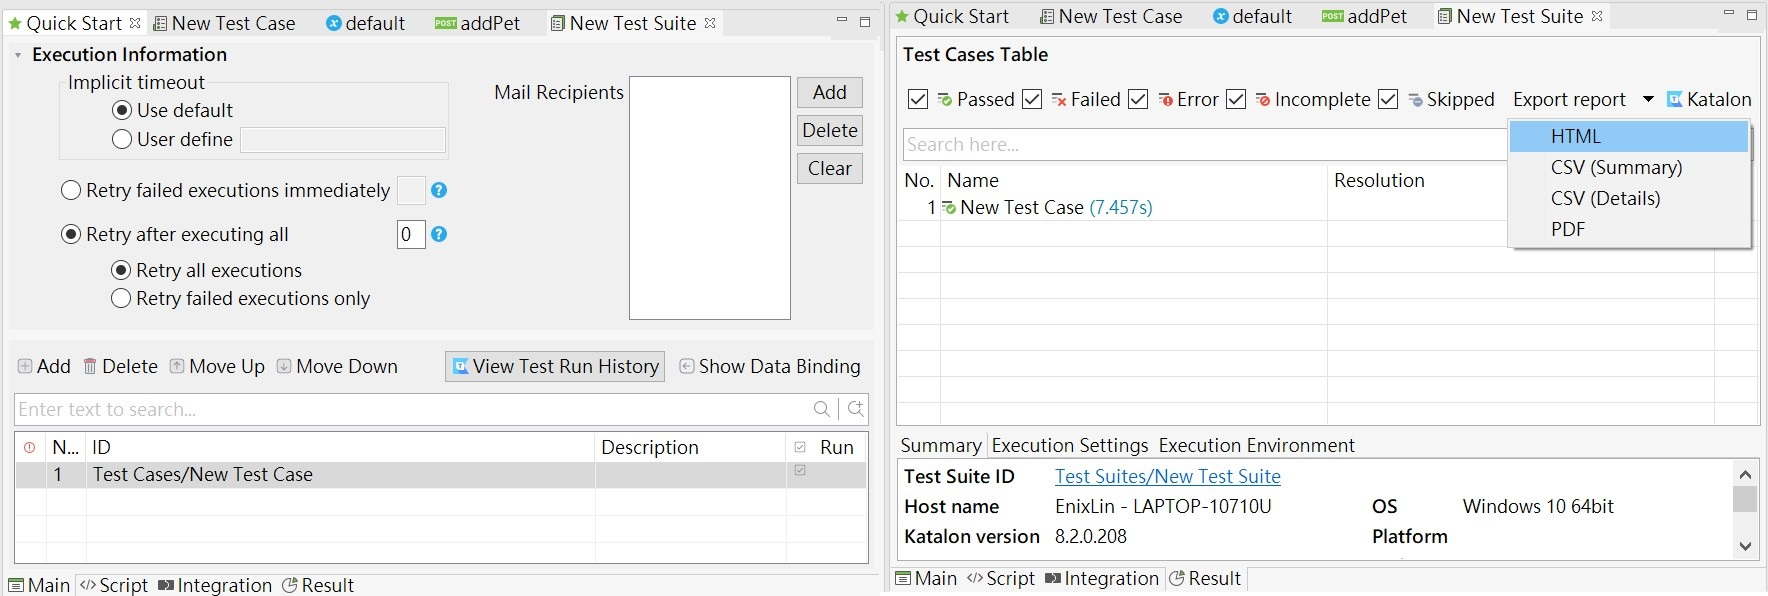
\includegraphics[width=1\textwidth]{picture/輸出報告.jpg}
\end{frame}
%----------------------------
\begin{frame}
    % \frametitle{Reports}
    \begin{center}
        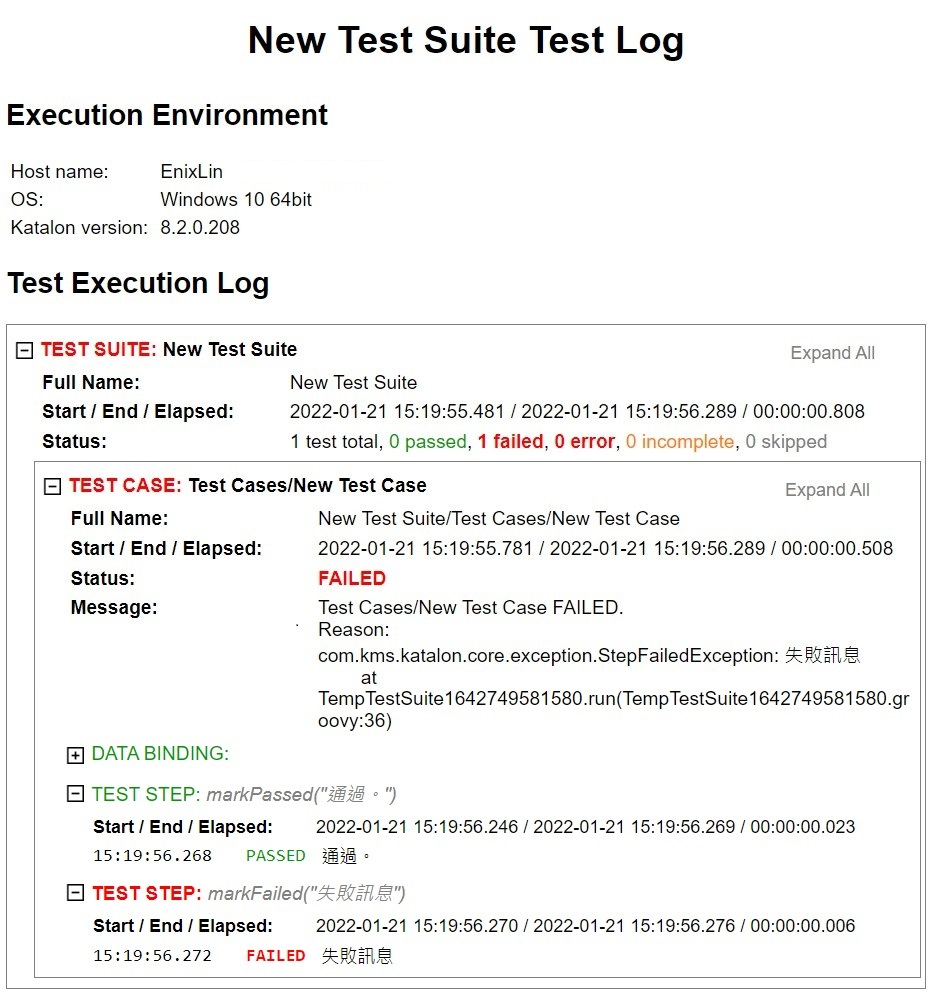
\includegraphics[height=0.95\textheight]{picture/reportHtml.jpg}
    \end{center}
\end{frame}
%----------------------------
\ifx\allfiles\undefined
\end{document}
\fi